\begin{savequote}[8cm]
The association of paternal and maternal chromosomes in pairs and their subsequent separation during the reducing division as indicated above may constitute the physical basis of the Mendelian law of heredity.
   \qauthor{--- \cite{sutton1902morphology}}
\end{savequote}

\chapter{\label{ch:2-SDA} Single Cell Transcriptomics}

\minitoc

\section{Experimental Data Generation}

The work and data described in this section was generated by Min Jung and colleges in Don Conrad's group.

The samples generated are as follows:

\begin{itemize}
	\item 11 wild type C57BL/6 mice
	\item 3 FACS samples (primary spermatocyte , secondary spermatocyte, and spermatid) from a 12th wild type
	\item C57BL/6 mouse
	\item 1 sample of FACS sorted spermatogonial cells from 5 wild type C57BL/6 litter mates
\end{itemize}

In addition to wild type mice four different mutant mice were included:
\begin{itemize}
	\item 6 Mlh3-/- B6;129 mice
	\item 2 Hormad1-/- B6;129 mice
	\item 2 Cul4a-/- B6;129 mice
	\item 2 CNP eGFP BAC TRAP C57BL/6 mice.
\end{itemize}

The cells were dissociated by two methods: enzymatic for the first two wild type mice and the spermatogonia and mechanical for the rest.

\section{Data Processing and QC}

The datasets described above were merged (54,251 cells and 38317 genes) and processed through a series of quality control and normalization steps:

Cells with fewer than 200 UMI counts or fewer than 50 genes expressed were removed. Cells were also removed if their total UMI count or number of genes expressed was more than 1 standard deviation below the mean for that experiment. A tSNE reduction of this dataset revealed an amorphous homogeneous group characterised by a low library size, high mitochondrial gene expression and often co-expressed genes from early and late meiosis suggesting poor quality and or doublet cells and so these were removed. Cells with a normalised mt-Rnr-2 expression of greater than 2 were also removed. After these steps 20,322 cells and 28,893 genes remained.

Genes in the lower third of expression means were then removed and cells were normalized by square root transformation of total transcript counts per cell and genes were normalized to unit variance. All expression values were capped to maximum of 10. This results in a final matrix of 20,322 cells by 19,262 genes with a sparsity of 93.8\% and a median UMI count of 1312 per cell.

SDA was then run with 50 components for 10000 iterations.

\section{Determining an appropriate reduction dimensionality}

When performing a dimensionality reduction such as matrix factorisation we must choose the number of latent components. Too low and we may miss some real components, too high and we may find spurious components due to overfitting.

We found when increasing the number of components 

\begin{figure}[H]
	\centering
	\includegraphics[width=\textwidth]{figures/single_cell_component.pdf}
	\caption{Component 4 is represents a single cell. A) Cell scores for component 4 ordered by value. B) Gene loadings for component 4. C) Predicted expression using only component 4 vs Raw Normalised Gene Expression. Pearson's correlation is quoted (equal to correlation with the gene loadings) . All of the genes with high expression in this cell have a high gene loading in this component. D) As in C but for the cell with the second highest association. The correlation is much lower. E) As in C but using all components except 4. The correlation is less than C especially for highly expressed genes. F) As in C but using all components for the prediction.  This is the sum of C and E}
	\label{fig:single_cell_component}
\end{figure}

\section{General Properties of Inferred Components}

By inspecting the change in free energy as well as the change in fraction of gene loadings with PIP < 0.5 we can confirm that the algorithm had converged within the 10,000 iterations for which it was run \ref{fig:SDA_diagnostics}.

As expected in line with previous reports from \cite{Hore2016Tensor} the PIPs have a bimodal distribution \ref{fig:SDA_diagnostics}.

In addition the gene loadings are very sparse with 79.8\% of the gene loadings having a PIP of less than 0.5. These genes have a tight distribution of loadings around 0 with a maximum absolute loading of 0.011 and 99\% of the loadings lying within the range (-0.0033, 0.0036). Of the gene loadings with a PIP of greater than 0.5 the maximum absolute loading is 1.31 and the mean is 0.062.

Five components have outlying maximum cell scores \ref{fig:SDA_diagnostics}. These components have a single high loading in one cell and likely represent over fitting of a component to a single cell and so are not considered in further analyses \ref{fig:single_cell_component}. Two components 42, and 17 have outlying maximum gene loadings, we will later see that these components represent pachytene and spermiogenesis respectively. 

\begin{figure}[H]
	\centering
	\includegraphics[width=\textwidth]{figures/SDA_diagnostics.pdf}
	\caption{Checking convergence of SDA. A) Change in free energy is often 0 by the 10,000th iteration. B) Change in fraction of PIP <0.5 is less than 0.005\% C) Distribution of maximum scores and loadings for each component. E) Distribution of PIPs across all components, showing expected bimodal distribution.}
	\label{fig:SDA_diagnostics}
\end{figure}

\section{Low Dimensional Visualisation}

Despite reducing the dimensionality of the original dataset from 19,262 to 50 this is still too high to visualise the overall structure of the data. This can often be achieved by performing a second non-linear reduction such as tSNE or UMAP (normally PCA is the linear reduction) \cite{maaten2008visualizing, mcinnes2018uniform, Etienne2018Dimensionality}. We find a horseshoe like effect often found when reducing datasets with an underlying 1 dimensional structure \cite{Novembre2008, Podani2002}. By looking at genes with known expression patterns from the literature we can induce that in this case that the linear structure is developmental time of spermatogenesis and that the clusters in the centre are somatic cells.

To generate a pseudo-timeline we used a similar approach to that implemented in SCUBA \cite{Marco2014-ky}. We iteratively fit a principal curve through the t-SNE plot with increasing degrees of freedom from 4 to 9 using the curve from the previous run as the starting point \cite{Hastie1989-ej}. Each cell was then assigned to the closest position on this curve. Somatic cells and the Hormad1 X-activated cells were excluded during pseudotime construction. Somatic cells were defined by thresholding on the cell scores of somatic components.

The order of components was determined by using a weighted mean of the pseudotime values, where the weights are the cell scores of the component. In addition only cells with an absolute cell score of greater than 2 contribute to the mean.

\begin{figure}[H]
	\centering
	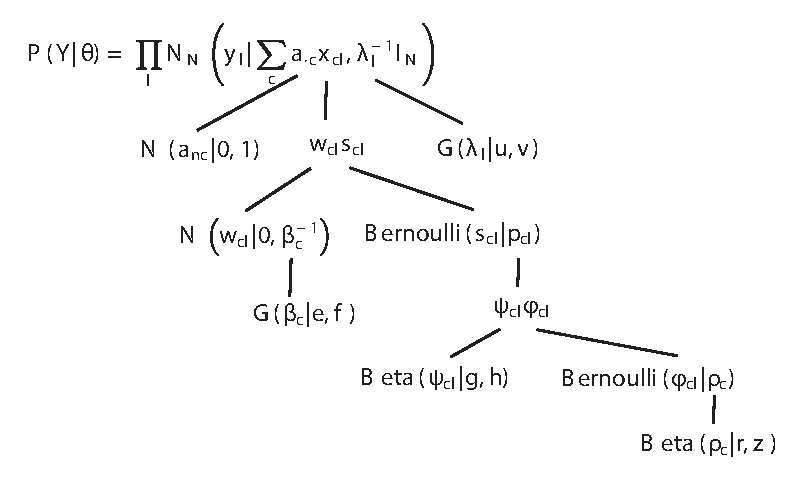
\includegraphics[width=\textwidth]{figures/SDA.pdf}
	\caption{}
	\label{fig:SDA}
\end{figure}

We can perform the same visualisation on the transposed cell scores or gene loadings to see how the components relate to each other. We find 7 major clusters of components, with hindsight these correspond to: 1) Spermatogonia, 2) Leptotene/Zygotene 3) Pachytene 4) Round Spermatid (Acrosomal) 5) Spermiogenesis 6) Somatic and 7) Somatic (Sertoli). We can see that our manual labelling of the components is consistent with the clusters.

\begin{figure}[H]
	\centering
	\includegraphics[width=\textwidth]{figures/tSNE_Components.pdf}
	\caption{A low dimensional representation of the components shows 7 clusters.}
	\label{fig:tSNE_Components}
\end{figure}



\section{Imputation}

Due to low input material and limited transcript capture efficiency the original data is very sparse. 

In the process of fitting the SDA model we have also effectively imputed the data. Multiplying out the cell scores and gene loadings matrix generates a matrix of the same dimensions as the original data but populated with the model's predicted values. Visualising these new expression vectors through pseudotime in comparison to the originals there are many fewer zero values when the gene is expressed as well as fewer outliers when it's unexpressed.

A problem with validating this imputation scheme is that we can't evaluate against the true value for each cell because we don't know the true values. Instead we partition the dataset by randomly assigning each original read to either a training or test dataset and then run SDA and imputation on the training dataset only. If the imputation is working then we should be able to predict the rankings of the gene expression in the test data.



As comparisons we either simply used the reads from the corresponding cell in the training dataset or an average over all cells. If we use the training data, we do ok for the highly expressed genes but then we run out of reads and basically guessing at random for the rest. Using an average we do better for the lower expressed genes, but of course if you take the average over all cells you may as well have done a bulk sequencing experiment. We can take the area under these curves to visualise comparative accuracy for all cells, compared to the cellwise training data we do almost allways better using the imputation, particuarly well when the library size is low. Using the average we also do almost always better, and best when the cell type is not like the average as you might expect.


\section{Components}

\subsection{Telocytes}

\subsection{Leydig Cells}

\subsection{Macrophages}

\subsection{Lymphocytes}

\subsection{Spermatogonia}

\subsection{Telocytes}

\subsection{Leptotene - Zygotene}

During meiosis there is an extended prophase I (lasting 14 days in mice), which is itself divided into a number of stages: Leptotene, Zygotene, Pachytene, and Diplotene. In Leptotene and Zygotene the homologous chromosomes undergo presynaptic pairing, aided by meiosis-specific cohesin, and Spo11 creates several hundred programmed double-strand breaks at sites bound by Prdm9, the only known mammalian speciation gene (Mihola et al., 2009). We find a component (5) in which many of the genes required for this process have high loadings, including Prdm9 itself, Spo11 partner Top6bl (Gm960) (Robert et al., 2016; Vrielynck et al., 2016), Dmc1 which is required for DNA strand exchange \cite{Brown2014-wg}, proteins involved in the loading of Dmc1: Brca2 \cite{Martinez2016-qj} and Tex15 \cite{Yang2008-nj} as well as  components of the meiotic cohesin complex Rad21l, Smc1b, Smc3, and Esco2 \cite{Rankin2015-jz}. (Figure 3C-D; Table S3).

This component is also highly enriched for GWAS hits of recombination rate in humans \cite{Halldorsson2019-vk}. Of the 24 significant GWAS loci identified with confidently associated causal genes, more than half (13) rank within the top 300 genes of this component, and almost all (20) rank within the top 1300 genes (p = 5.2x10-18, OR = 77.8 [95\% CI:36.4,Inf] and p = 2.4x10-20, OR = 70.1 [95\% CI:26.9,Inf]] respectively by fisher's exact test [FET], Figure 3F). One of the hits, Msh4, is not ranked highly in this component (2734th out of 19262), however, it is known to function as a heterodimer with Msh5, which ranks 34th \cite{Rakshambikai2013-qi}. This highlights one of the advantages of single cell RNAseq compared to GWAS for target discovery in that it does not rely on the presence of (perhaps rare, small effect) genetic variants. In addition it directly provides a list of genes rather than SNPs affecting unknown causal genes, For example the previous GWAS had identified a SNP in the intron of Ccdc43, however our expression data strongly suggested the adjacent gene Meioc as the causal gene (ranked 183rd vs 13,651st in component 5) in addition to the subsequent reports that Meioc is responsible for maintaining an extended meiotic prophase \cite{Abby2016-kc, Kong2014-ae, Soh2017-vq}. 

The strong enrichment of genes involved in recombination in this component suggests other highly ranked genes of unknown function could also play key roles in this process. This proved to be the case for two such genes during the preparation of this manuscript. Firstly Ankrd31 (ranked 102nd) was found to control the number, timing, and location of double strand breaks in meiosis \cite{Boekhout2018-wr, Papanikos2018-jp} and Hsf2bp (now Meilb2, ranked 194th) was found to be a master regulator of meiotic recombinases \cite{Zhang2019-fb}.


\subsection{Pachytene}
During zygotene the paternal and maternal homologues pair with one another in preparation for recombination in pachytene. When partners fail to synapse they are marked by HORMAD1, HORMAD2 and BRCA1. This is followed by recruitment of ATR and the creation of $\gamma$H2AX resulting in transcriptional silencing (Meiotic Silencing of Unsynapsed Chromatin). As the X and Y chromosomes are only partially homologous they fail to fully synapse and are silenced by this processes (Meiotic Sex Chromosome Inactivation, MSCI). We are able to clearly see this effect in the ratio of X to autosomal expression through pseudotime (Fig \ref{fig:MSCI}) We can also see this in the gene loadings of pachytene components with an almost complete lack of loadings on the sex chromosomes.

\begin{figure}[H]
	\centering
	\includegraphics[width=\textwidth]{figures/MSCI.pdf}
	\caption{}
	\label{fig:MSCI}
\end{figure}

In addition to MSCI we are able to address another curiosity of spermatogenesis with this data - cytoplasmic sharing. From the mitotic divisions of the spermatogonia onwards cytokinesis does not fully complete and $um$-wide cytoplasmic bridges are formed between adjacent cells such that the cytoplasm could be shared across a synctium of cells \cite{Greenbaum2011Germ}. Whilst theoretically thousands of cells could be connected in practise up to 650 connected cells have been observed \cite{ren1991clonal}. The extent to which mRNA sharing occurs is unknown although it has been shown for individual genes \cite{braun1989genetically}. As post-meiotic cells are genetically haploid if there was not widespead sharing we might expect to see two populations of cells, those with more X transcripts and those with more Y. However for both X and Y we do not observe a splitting suggesting the transcripts, at least on the X and Y, are efficiently shared.

There remains a possibility that some individual or group of genes are not shared, such as has been observed for autosomal genes in a mutant heterozygous context: the t-complex responder mutant (SmokTcr) which functions as an antidote in the poison-antidote meiotic drive system of the t-complex \cite{Veron2009retention} and Spam1 which causes transmission ratio distortion in Robertsonian (Rb) translocation-bearing mice \cite{martin2005spam1}.

% Haploid Cytoplasmic Sharing

\subsection{Hormad1 X Chromosome Activation}
In addition to some components with lack of loadings on the sex chromosome there is also a component with an \textit{excess} relative to the autosomes. This component is active exclusively in a subset of Hormad1 KO cells positioned in zygotene stage. As previously mentioned HORMAD1 marks unsynapsed chromosomes, when HORAMD1 is completely absent as in the KO it appears as though the sex chromosomes are fully synapsed and so they fail to be transcriptionally silenced. We find that not only does Hormad1 KO fail to silence previously expressed sex-linked genes, many previously \textit{unexpressed} sex-linked genes such as Rhox2h have high expression. Interestingly, there are also multiple autosomal genes with high loadings. This may be due to ectopic expression of sex-linked transcription factors; for example, Zfy1 and Zfy2 were previously shown to cause pachytene arrest when misexpressed \cite{royo2010evidence}. We find a very strong association between genes in this component and genes overexpressed in mice which have mutations in either Hormad1 ($p<10^{-35}$) or Trip13 ($p<10^{-150}$) \cite{ortega2016surveillance}.


\subsection{Meiotic Divisions}

\subsection{Round Spermatid}

\subsection{Spermatocytes}

\subsection{Respiration}

As well as meiotic specific processes we found components with broader functions such as respiration. Component 9 contains 41 out of 57 of the respiratory complex I, III, and IV genes (complex II is an alternative pathway) (p = 7.4x10-53, OR = 104 [95\% CI: 62.1,Inf] FET).

\subsection{Batch Effects}

In addition to transcriptional programmes we 

\section{Motif Inference}

\subsection{Enrichment of Known Transcription Factor Targets}

\subsection{\emph{De-novo} inference form promoter sequences}

\subsection{Novel Motifs}

\subsection{Broad-scale patterns of TFBS occurrence over PseudoTime}

\subsection{Patterns of CpG occurrence}

Given there exists these groups of co-expressed genes the obvious question is what's driving this expression? One major class of transcriptional regulation is the binding of transcription factors to promoters and enhancers.

There are some transcription factors that are known to regulate meiotic gene expression. One of these is MybA (encoded by Mybl1) and we find that the predicted direct targets of the MybA transcription factor as found by ChIPseq and RNAseq of KO mice we find that they are strongly enriched specifically in the pachytene components as expected based on what's known about MybA. The story is similar for other known meiotic transcription factors Stra8, Rfx2, and Crem.

If these transcription factors were regulating the co-expressed genes we would expect to see enrichment of their binding motifs in those genes. However, it is possible that there are undiscovered transcription factors and so instead we inferred \textit{de novo} motifs from the promoter sequences of the top genes from each component. 

This resulted in 16 groups of motifs including matches to Stra8, Mybl1, Rfx2, and Crem. To gain a broader view of which components these motifs act on we computed the linear association between the gene loadings and the motif presence probability for each motif-component combination. In addition to some relatively specific enrichment (e.g. Stra8 in Leptotene C5, Mybl1 in Pachytene C42, and Rfx2 in Acrosomal C30), this revealed an obvious “switch” with one group of transcription factors appearing to regulate early meiosis (prior to the meiotic division), and another group regulating meiosis post-division. Moreover, most meiotic motifs spanned several components. This implies that promoter motifs might offer “broad-scale” control, but differences at “fine scales” among individual components might instead be largely driven by TF binding to more distant enhancer regions, mRNA degradation by microRNA, or other post-translational mechanisms. Hence, additional work will be required to fully delineate the mechanisms controlling meiotic transcription.

As we inferred these motifs de novo we were able to discover previously unknown motifs. Indeed, we identified a motif with similarity to the ATF1/CREM motifs in the late components, but with the addition of a CAA tail and lacking the central G nucleotide which would otherwise form a CpG dinucleotide (Figure 5A). We hypothesise that, plausibly, this may represent the binding motif of the tau isoform of CREM known to be active in late spermatogenesis (Sassone-Corsi, 2000). Consistent with the more general pattern of CpG occurrence we find this ATF1/CREM-t motif highly associated with post-division components; in fact it is the most strongly associated motif in multiple such components (Figure 5B). In addition, the STRA8 motif, whilst it has a poor match to any motif in the HOCOMOCO database, is the same as the recently discovered motif from Stra8 ChIPseq experiments (Kojima et al. 2019).



Almost all of the motif acting pre-meiotic division include a CpG in their motif, and none of the post division motifs do, so there sees to be this broad switch between classes of TF during meiosis. Indeed we found an even stronger pattern of association simply using the count of CpG occurrences.



\subsection{Limitations \& Extensions}
Clustering of the transcriptome with respect to meiotic stage is frustrated by promiscuous transcription~\cite{Soumillon2013Cellular} and post-transcriptional regulation. For example Prm1 (Protamine 1) and Smcp (Sperm Mitochondria-associated Cysteine-rich Protein) mRNA are stored for three and seven days respectively as free ribonucleic particles before they are translated into protein on polysomes~\cite{Cullinane2015Mechanisms, Kleene1984Translational, Kleene2004Patterns}.

%This widespread uncoupling of transcription and translation is required due to the cessation of transcription in late spermatids when the nuclear DNA is compacted. 

%However this obviously frustrates attempts to identify cell types from mRNA \emph{expression} given information on protein \emph{function}. There is also widespread promiscuous transcription in testis which increases the noise levels in an a dataset with an already low signal to noise ratio.

One important next step will be to compare our results to previously published datasets from bulk-RNAseq profiling in the testis where it is possible to perform orthogonal experiments such as immunohistochemistry in order to determine cell stages.

%  it may also be possible to assess the extent of cytoplasmic sharing through intercellular bridges in post-meiotic spermatocytes via hemizygosity of SNPs / monoallelic expression~\cite{Greenbaum2011Germ, Hoffmann2016TransposonBased}.

With the transcriptional profile of meiosis is known it may be possible to deduce the gene regulatory network by incorporating the temporal expression information with an analysis of DNA sequence motifs and prior information of known transcription factors involved in meiosis~\cite{PadovanMerhar2013Using, Goutsias2007Computational}. Methods previously used for such purposes include ARACNE, WGCNA, iRegulon, and Boolean regulatory networks~\cite{Margolin2006Reverse, Zhang2005General, Janky2014IRegulon, Moignard2013Characterization}.

Ultimately these analyses provide hypothesis in the form of new genes involved in meiosis. These predictions could be tested using an orthogonal experimental technique for example RNA in situ hybridization to confirm cell and stage expression profiles~\cite{Moffitt2016Highperformance,Choi2016Mapping}, and or gene knockouts to confirm functional importance in meiotic processes~\cite{Jamsai2010Mouse}.
